\section{Implementation of SemNotes}
\label{sec:semnotesimplementation}

In the development of SemNotes, we tried to reuse as much as possible of the features provided by the host Semantic Desktop, Nepomuk-KDE\@. Using the existing functionality enabled better integration with the rest of the system, while reducing the effort required for the implementation. Nepomuk-KDE provides out of the box central RDF storage for the desktop, and an efficient means to access and query the data. 

We describe below the implementation of each of the modules introduced in the design section. 

\subsection{Data Representation} 
\label{sub:datarepresentation}

We describe the data created by SemNotes using a subset of the desktop ontologies described in Section \ref{sub:nepomuk} --- Personal Information Model (PIMO) and Nepomuk Annotation Ontology (NAO). 
Figure~\ref{fig:holiday} shows a basic note with metadata, and Listing \ref{lst:noterdf} contains the Turtle representation of the same example. 

The central unit of information handled by SemNotes is the note --- represented as an instance of \verb|pimo:Note|. 
The information stored for each note consists of: 
\begin{itemize}
 \item title --- \verb|nao:prefLabel|
 \item content --- \verb|nao:description|
 \item creation date --- \verb|nao:created|
 \item last modification date --- \verb|nao:lastModified|
 \item rating --- \verb|nao:numericRating|
 \item tags --- \verb|nao:hasTag|
 \item related desktop resources --- \verb|pimo:isRelated|
\end{itemize}

The Nepomuk ontologies make the distinction between resources representing native computer structures, which are described with the Nepomuk Information Element (NIE) ontology and resources representing concepts in the real world, which are described with the Personal Information Model (PIMO).

Before representing the PIMO concepts, most of the semantic data on the desktop is extracted from \verb|nie:DataObject|s and interpreted as \verb|nie:InformationElement|s. This is due to the fact that generally the information is still created by non-semantic applications, and to make it useful to the Semantic Desktop it has to be transformed, while keeping provenance information and feeding back into the applications that created it.

The extra step of extracting resources is not needed in the case of the information created directly for the Semantic Desktop by semantic applications. Thus, if no data is stored outside of the repository, no NIE resources are created. This is a characteristic of SemNotes and of other semantic applications for the Semantic Desktop.

The \verb|pimo:Note|s created with SemNotes can however be exported as text or HTML files, for backup or other purposes, thus associating a NIE resource to a note. This is the reverse of the usual process, and the change stems from working directly with the framework provided by the Semantic Desktop.

\begin{figure}[th]
 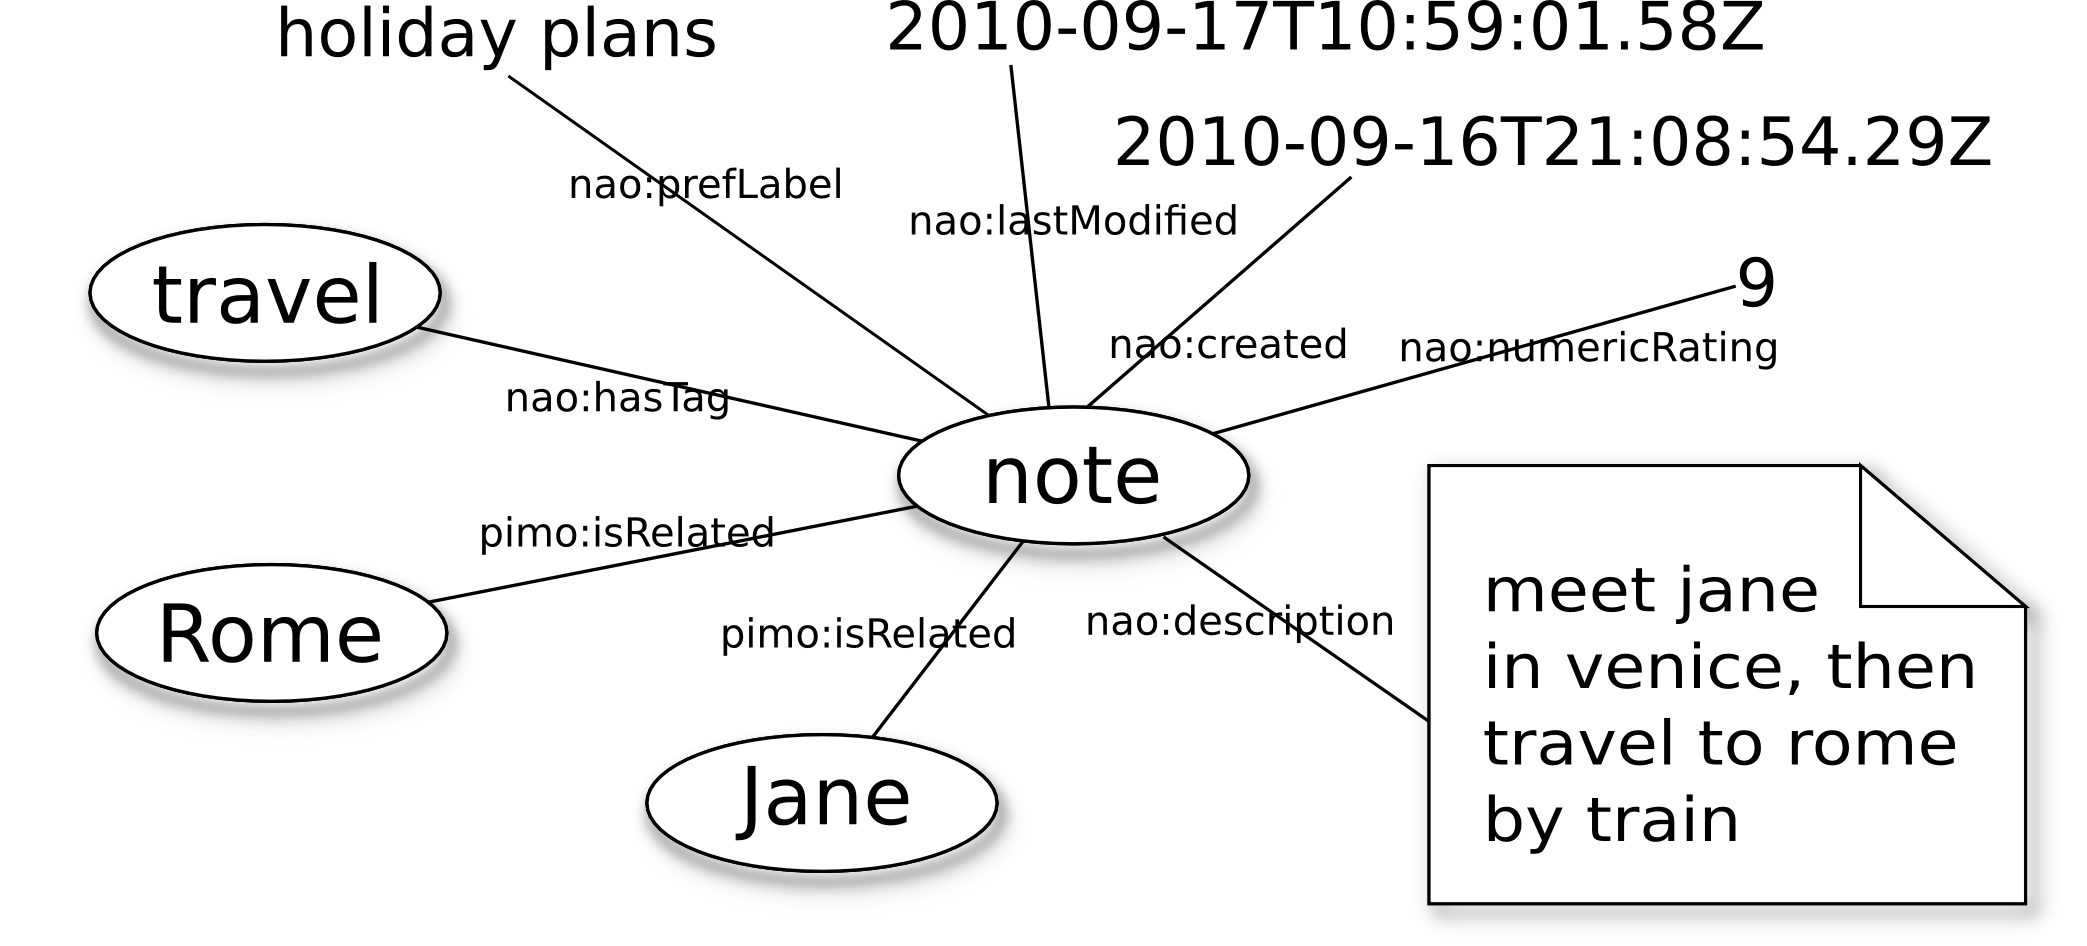
\includegraphics[width=0.9\linewidth]{chapters/core/img/note-properties}
\caption{Graph representation of the information about a note.}
\label{fig:holiday}
\end{figure} 

\subsubsection{Note metadata}

Tagging, rating and commenting are basic features provided out of the box by the Nepomuk-KDE system, for all types of resources. 
In SemNotes the only categorisation mechanism we use are tags, preferring simplicity over the more accurate mix of categories, topics and tags. The \verb|nao:hasTag| relation links the note to system-wide tag instances, thus enabling the reuse of tags throughout all applications, reducing duplication of classification work for the user. 

We later added support for rating to the interface, leaving the meaning of the rating open for the user to decide --- some possible examples include importance, urgency, quality of the content, or readiness for publication (in the case of a draft blog post as will be shown in Chapter \ref{ch:mischelperapps}).

Commenting on notes, although supported by the underlying system, because notes are resources, is not supported in the interface of SemNotes. We made this decision because the notes are themselves a type of comment, and we considered the feature redundant. 

\lstset{
	caption={RDF representation of a note.}, 
	label=lst:noterdf,
	language=turtle
}
\setlength\parindent{0in}
\begin{minipage}[t]{\linewidth}
\begin{lstlisting}
@prefix xsd: <http://www.w3.org/2001/XMLSchema#> .
@prefix pimo: <http://www.semanticdesktop.org/ontologies/2007/11/01/pimo#> .
@prefix nao: <http://www.semanticdesktop.org/ontologies/2007/08/15/nao#> .

<nepomuk:/res/thenoteuri> a pimo:Note ;
       nao:prefLabel "holiday plans"^^xsd:string ;
       nao:description "<html>...</html>"^^xsd:string ;
       nao:created "2010-09-16T21:08:54.29Z"^^xsd:dateTime ;
       nao:lastModified "2010-09-17T10:59:01.58Z"^^xsd:dateTime ;
       nao:numericRating "9"^^xsd:int ;
       nao:hasTag <nepomuk:/res/travel> ;
       pimo:isRelated <nepomuk:/res/Rome>, <nepomuk:/res/Jane> .
\end{lstlisting}
\end{minipage}
\setlength\parindent{0.21in}

\subsubsection{Note content}

Because notes are generally short \cite{Bernstein2008} we decided to store the note content in the RDF repository, as a property of the note (\verb|nao:description|). The value is the HTML string representing the content of the note, including formatting. This decision enables us to use the indexing and full text search feature provided by Nepomuk-KDE. 

Using the general property \verb|nao:description| to store the content of the notes, opens up the possibility of treating any semantic resource on the desktop as a note in SemNotes. This is equivalent to adding comments on each resource, but employing the functionalities provided by the application, including the analysis of the text to suggest relations. This enables serendipity --- discovering non-obvious connections between any desktop resources.

\subsubsection{Related resources}
 
As we discussed, the most important feature of SemNotes is the interlinking of notes with relevant resources from the desktop. The relations are stored using \verb|pimo:isRelated|. In the current revision of SemNotes, this is the only type of relation. This decision was based on the results of the long term study of Gnowsis usage \cite{Sauermann2008} which found that for PIM tasks it is enough to express that two things are related, and that the simpler properties are preferred by users over the more specific ones, regardless of the possible loss of meaning. However, we consider extending the range of possible relations in future versions. Having the information about the resources that are linked, specifically about the type of the resources, we can infer the possible relations to suggest, based also on knowledge from the desktop ontologies. 

Restricting the types of possible relations also keeps the interface simple, which was one of the design goals, and one of the biggest challenges we encountered, as we show in more detail in \ref{sub:semnotesvisualization}. We further explain the extraction and creation of relations in \ref{sub:interlinking}.

\subsection{Data Management}
\label{sub:datamanagement}

SemNotes supports all the phases of the note life-cycle.

When a new note is created, a new URI is generated for it, and the creation time is set. The rest of the properties are not set at creation time. As note data is added (i.e. the refinement phase), the metadata about the note and the content is updated. At each new update or annotation of the note, the last modification date is also updated. The notes can be found (i.e. the access phase) through full-text search, filtering by tags, related resources, and by creation date. Once the required note is found, it can be viewed in the editor. When a note is deleted, all metadata and relations about it are deleted as well, however, none of the tags and related resources are removed from the system, as they might originate from, or be used by other applications. The publication phase is also supported by SemNotes, as notes can be exported as HTML or text files, or even directly published online as blog posts \cite{Dragan2010a}.

As mentioned above, SemNotes uses the RDF repository provided by Nepomuk-KDE for all data storage. 

\subsection{Interlinking}
\label{sub:interlinking}
The interlinking of notes with related resources is the key feature of SemNotes. This feature realises the actual integration of the new information with the existing network of linked desktop data. Annotating the notes with related information captures the context of the note. Context is important for personal information management because it enables reminding and better (more precise, faster) search. Links between resources also support wayfinding \cite{Jones2008KFTFBook} and encourage exploratory browsing and serendipity.

The module uses entity recognition and string matching algorithms to detect and suggest possible related resources, but no link is created until the user selects the correct one. This mixed-initiative approach is a compromise between the precision of the links created and the amount of interference with the user's workflow.

The current implementation suggests annotations based on the knowledge about existing desktop resources, using entity matching techniques to identify the likely candidates. Certain types of resources are more likely to be related to notes (e.g. people, organisations, projects, events, tasks, other notes, locations). By default, SemNotes restricts the search for suggested resources to these types, but the user can easily modify the list. We do not include every resource on the desktop because of the large number of files that are indexed by the Semantic Desktop, which would clutter the suggestion list. For the resources of the given types, all textual properties are compared against the note text. This way, resources that do not explicitly have the search term in their label will show up in the suggestion list. An example is shown in Figure~\ref{fig:annotation}: for the word ``John'' other notes that mention him are suggested, even though his name is not present in the label.

\begin{figure}[tb]
 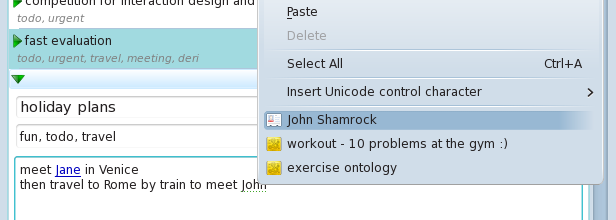
\includegraphics[width=\linewidth]{chapters/core/img/semnotes-screenshot-menu}
\caption{SemNotes annotation suggestion and link.}
\label{fig:annotation}
\end{figure} 

SemNotes does not currently offer suggestions based on online resources\footnote{Similar to \url{www.zemanta.com}.}, unless there is a desktop resource previously created for the relevant Web data (i.e. a bookmarked Web page becomes a desktop resource). 

We are working on an information extractor module, which identifies new information in the content of the notes. It will suggest the creation of new desktop resources from the text, like events, tasks or contacts, that will then be linked to the note. 

Since the annotation suggestions are computed while the user types the note, efficient processing is required. The process of finding possible matches follows:
\begin{enumerate}
 \item Scan the text and identify possible candidates represented by a single word or a sequence of words.
 \item For each possible entity found in the text find a list of existing desktop resources that match it. We use string matching to compute a score for each resource found. The score takes into account the length of the matched string, and if the resource has been linked to the note before.
 \item Sort the matches by score and present them to the user in a non-intrusive way (see Section \ref{sub:semnotesvisualization}).
 \item If the user chooses any of the presented suggestions 
  \begin{itemize}
   \item create a link between the piece of text identified as an entity and the actual resource it represents.
   \item use the selected suggestion in the recalculation of the scores for the entities found for the rest of the note. Once a note is linked to a resource, that resource is more likely to appear again, and therefore it will be ranked higher.
  \end{itemize}
 \item If the user ignores the presented suggestions, no links are created, but the possible matches are saved for later use.  
\end{enumerate}

For the purpose of establishing context, and for organising notes, it is sufficient to create a single link between a note and a resource it is related to, regardless of how many times that resource is mentioned in the content of the note. Therefore the relation between the note and the desktop resource is created only once in the repository. However, if the note is viewed in SemNotes, all the links that the user created to the related resource are displayed.

The interlinking module also manages the removal of links between notes and desktop resources.
Because the suggestion of related resources is based on the content of the notes, once the last textual link to a related resource is removed, so is the relation between the note and the respective resource. 

SemNotes also supports the manual creation of links between the note and desktop resources that are relevant but have no explicit mention in the text.

\subsection{Visualisation}
\label{sub:semnotesvisualization}

SemNotes displays the notes as a list that can be sorted by title, creation or last modification dates, or rating. Each note can be opened in-list for quick access, or maximised over the entire window, for viewing and editing. In the in-list mode, several notes can be open and edited at once (see Figures \ref{fig:screenshot} and \ref{fig:screenshot2notes} for the current version of the SemNotes user interface.).

\begin{figure}[tb]
 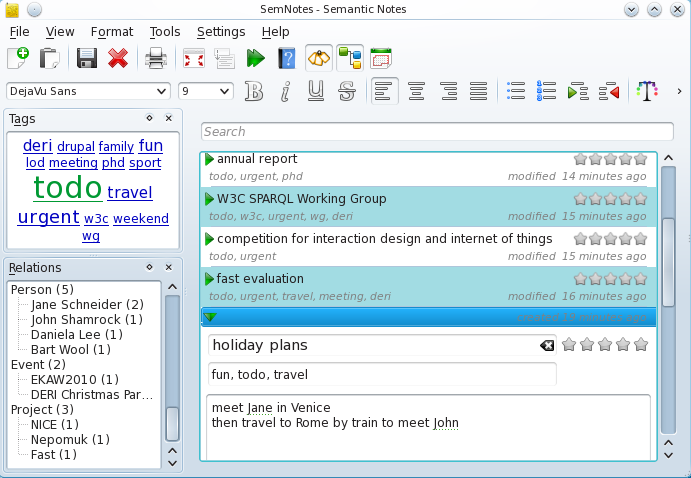
\includegraphics[width=\linewidth]{chapters/core/img/semnotes-screenshot}
\caption{Current version of the SemNotes user interface.}
\label{fig:screenshot}
\end{figure} 

\begin{figure}[tb]
 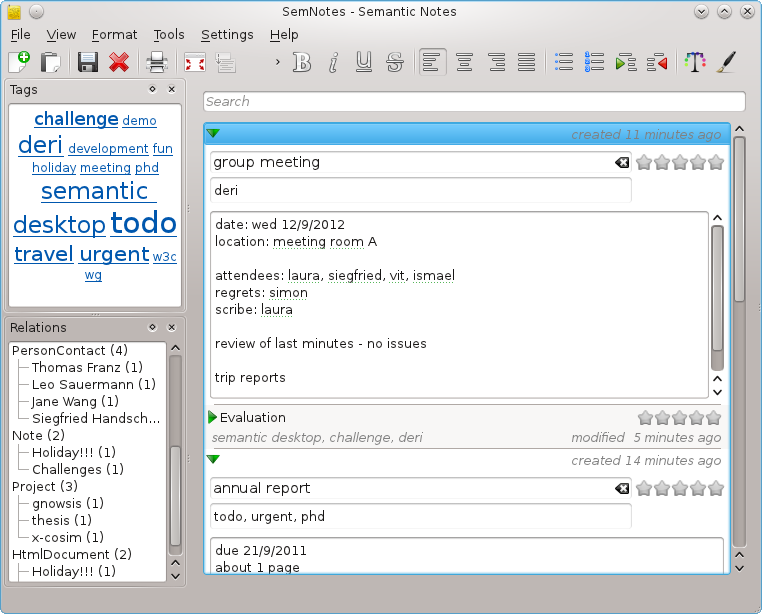
\includegraphics[width=\linewidth]{chapters/core/img/semnotes-screenshot_2notes}
\caption{SemNotes main window, with two notes open in-list.}
\label{fig:screenshot2notes}
\end{figure} 

An aggregated view of the list of notes is based on a restricted set of properties that the notes have in common. Depending on the set of properties used (one or more), the most suitable visual representation of the aggregated view varies. Currently SemNotes offers a tag cloud, a timeline and a related-resource view; each view aggregates information about the notes based on a single property (i.e. the tags associated, the creation date and the related resources, respectively). Aggregated views are displayed adjacent to the list of notes, and can be hidden by the user to allow more space for editing. 

These views also act as a custom faceted browser, as they provide filters on the list of notes. Filtering the list is as easy as clicking on a tag, time interval or related resource. A full text search box also acts as a filter on the list of notes, highlighting the search keywords in the content of open notes, if found. Multiple filters can be set at once, of mixed types. Figure~\ref{fig:screenshot} shows SemNotes with the tag cloud and related-resources views visible, and a tag filter set. A note is open in-list for editing. 

The editor component provides rich text editing of the note content, as well as easy editing of the note metadata. Tagging provides auto-completion based on all the tags on the Semantic Desktop, and creating a new tag is done just by typing its label. If the user does not set a title, SemNotes automatically sets it to the first line of the note. For the rating we used the default visualisation provided by the Nepomuk-KDE libraries, for a uniform interface across the desktop. The creation and last modification dates are the only metadata which cannot be changed through the user interface of SemNotes, as these properties are set automatically. They can be tweaked by expert users, by accessing the RDF repository directly. 

The suggestions for annotations are presented in a simple non-intrusive way, in the ``spell-checker'' style (i.e. the words for which suggestions were found are underlined with a green dotted line instead of a red squiggly line), and are available as context menu items, by right-clicking. Figure~\ref{fig:annotation} depicts how annotation suggestions are presented, and how a linked resource is displayed in the note. To remove an annotation is just as easy as creating it --- through a context menu item.

This presentation of the suggested resources is the result of several iterations of design, each improving on the previous one. 

\begin{figure}[tb]
 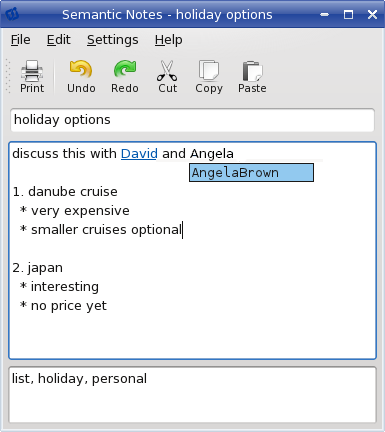
\includegraphics[width=0.6\linewidth]{chapters/core/img/linkednote_v1}
\caption{First version of the SemNotes note editor with pop-up style annotation suggestion.}
\label{fig:popup}
\end{figure} 

The first iteration relied on localised pop-ups with labels of the suggested resources, in the style of text auto-completion (see Figure \ref{fig:popup}). The style worked well when typing the text, and it also enhanced the speed of writing through the auto-completion it provided. The type of annotation of the text during its creation is called latent annotation \cite{Davis2010}, and it is an improvement over the two-step process of first creating the content and then annotating it. Depending on the text of the note, the pop-ups could appear often and distract the user, but they could be dismissed by continuing to type. However, when portions of text were pasted in the editor, several pop-ups were generated at the same time, which was confusing and did not allow the users to make all the connections they would. Changing slightly the pop-ups to only be displayed one-by-one when text was pasted proved not to be a good solution either, as in the case of large paragraphs it would take a long time and many mouse 
clicks for the paste operation to finish, thus interfering with the flow of work. 

Not just the interlinking support was changed from the first version of the application, but the entire user interface. The major redesign was supported by a usability study done as part of the Season of Usability\footnote{\url{http://openusability.org}} 2009, by Daivee Patel, a Human-Computer Interaction student at Drexel University, Philadelphia, USA, with the mentoring help of usability expert Paul Hibbitts of Hibbitts Design, Canada\footnote{\url{http://paulhibbitts.com}}. 
The goals of the project were to recommend changes to improve and/or redesign the SemNotes user interface based on analysis and user research methods, and to perform a usability evaluation of the new changes with a range of users to validate the design recommendations. 

The initial step of the project aimed at forming an understanding of what activities and tasks a user would perform with a note-taking application. This led to the use of a specific technique of task analysis called the activity grid based on the Activity Centred Design methodology. Using this method, we obtained a list of possible activities associated with using a note-taking tool, and each activity was subdivided into the tasks required to perform that activity and each task could then be further subdivided into possible actions. As the tasks became clearer, we identified the tasks that were relevant to SemNotes. These tasks helped focus the effort on the main usability issues and design specifically to address existing issues. 
A comparative analysis of five popular note-taking applications was conducted to help build a knowledge base for reference during the usability inspection of SemNotes. Each of the applications had their own unique features yet certain key functionality appeared standard across these kinds of applications. The examination proved helpful in determining the elements for redesign of the interface. 

The usability inspection of SemNotes was performed to identify usability issues with the existing interface that could be captured without the need to user test before the redesign.
Since the redesign was going to be based on key tasks or activities, we used a heuristic evaluation to identify top level issues.
The criteria for evaluation was the ISO standard ISO 9241\cite{ISO9241}, the principles associated with this standard are based on research and have the benefit of international consensus.
The results of the evaluation were used to help identify areas in the user interface most in need of design improvements, and to create a set of low fidelity mockups. 

A series of usability tests were conducted using the paper prototyping method to validate the initial recommendations for the interface redesign. During each testing session, participants were asked to think aloud and point to elements on the illustrated paper-based screen that they would click or look at based on the tasks provided. No assistance was provided to the users during the testing sessions. The usability test participants were selected via a screening survey on the criteria of experience with computer-based note-taking applications and note-taking habits. 
Based on the feedback from the first set of four users, the mockups were revised for the second round of usability testing while the tasks remained the same. The designs were further enhanced based on the 
feedback received in the second round. 

\begin{table}[htp]
\centering
\ra{1.3}
\begin{tabular}{p{0.45\linewidth} p{0.45\linewidth}}
\toprule
\textbf{Recommendation} & \textbf{Rationale} \\

\midrule
Multi Document Interface (presented as a single window with multiple panes) & By providing all key functionality within a single window, users did not have to manage multiple application windows.\\

Retain optional linking of text within linked editor via use of existing functionality (to click outside the auto complete pop-up) but to be supported by use of icons to indicate the type of resource being linked too & Users showed concern over unwanted text being linked. \\

Search should support searching by tags  & Users realised that since the notes were already tagged during creation, they would like to search by tags for better results. \\

Sorting of notes and tags in the left pane & Multiple options for sorting would help users in locating specific notes and/or tags. \\

First user experience should be provided & Learning curve associated with new applications -- having some introductory information and instructions in the opening screen will be useful. \\

\bottomrule
\end{tabular} 
\caption{Final recommendations for the redesign of SemNotes user interface, based on the usability study.}
\label{tab:sourecommendations}
\end{table}

Based on the accumulated results and feedback, we created a high fidelity mockup of the design, which included all the recommendations (see Table~\ref{tab:sourecommendations}) made as a result of the project, and which were incorporated in the second version of SemNotes.
The next iteration of the display for the annotation suggestions featured a side panel for each of the note edit boxes (see Figure \ref{fig:sidepanel}). The side panel proved to create less interference with the user's workflow, although the suggestions became less obvious. The panel presented the suggestions as a list of resources, that when clicked would highlight the parts of the content to which they were relevant. This helped the users understand from where the suggestion stemmed and if it was indeed correct. To create a link between the note and a suggested resource, the user had to right click on the corresponding item in the list and select ``Link''. Resources could also be removed from the suggestion list, and never be shown again for the current note, to help clear the list from overpopulating. This interface shifted the initial latent annotation style of SemNotes, back to a classic two-step process. Although the suggestions were still computed on the fly, as the user typed or pasted new text, 
because they were out of focus, users were inclined to leave the annotation step for later. Another issue of the side-panel variant was that it limited the screen real-estate for the most important function of SemNotes, that of note-taking. 

\begin{figure}[tb]
 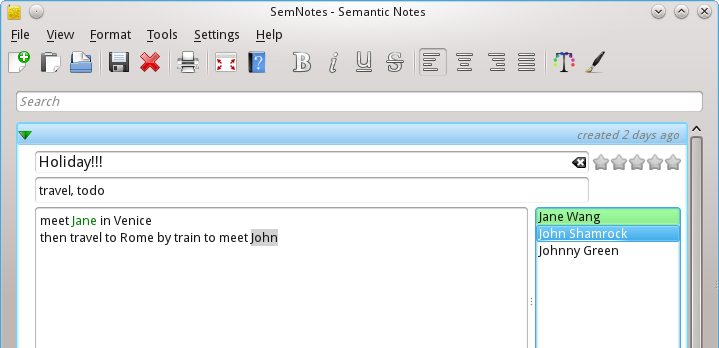
\includegraphics[width=\linewidth]{chapters/core/img/linkednote_v2}
\caption{Second version of the SemNotes note editor with a side panel to display the annotation suggestions.}
\label{fig:sidepanel}
\end{figure} 

To keep more of the screen space for the note editor, in the next iteration, we have abandoned the side panel in favour of the ``spell-checker'' type of notification. It is a mix of the first and second iterations, by giving the users the immediate feedback of the pop-ups, through the green dotted line that underlines words, while being unobtrusive in the note-taking activity. The suggestions are computed on-the-fly like before, but they are only shown if the user right-clicks on the underlined word or words, in keeping with the spell-checker metaphor.

The three iterations of user interface design have improved significantly the usability of SemNotes, as well as the ease of interlinking. However, further usability testing is needed to determine whether and how different types of relations can be created between the notes and the related desktop resources. 
